%% Week 36 -- Tuesday session (flipped classroom)
%% Companion to week36slides.tex (Monday lecture).  Two cases only this week,
%% by design: the bias-variance decomposition via the bootstrap, and k-fold
%% cross-validation for the Ridge penalty -- extended (2026-09-01) with the
%% full selection recipe of book Section 3.14: standard errors, the
%% one-standard-error rule, refit, test set once, Lasso vs Ridge, and
%% cross-validation vs the bootstrap.  No warm-up frames: the first twenty
%% minutes are open questions from Monday.  The cases are worked in
%% week36tuesday.ipynb.
%% Build:  pdflatex week36tuesday.tex  (twice)
\documentclass[10pt,aspectratio=169]{beamer}
\usetheme{red_plain}
\usepackage[T1]{fontenc}
\usepackage[utf8]{inputenc}
\usepackage{amsmath,amssymb,bm}
\usepackage{graphicx}
\usepackage{listings}
\usepackage{xcolor}
\usepackage{booktabs}
\graphicspath{{../BookFigures/chapter02_statistics/}{./}}

%% ---- code listings
\definecolor{codebg}{rgb}{0.97,0.97,0.97}
\lstset{language=Python,basicstyle=\ttfamily\scriptsize,backgroundcolor=\color{codebg},
  keywordstyle=\color{blue!70!black}\bfseries,commentstyle=\color{green!45!black},
  stringstyle=\color{red!60!black},showstringspaces=false,frame=single,
  framerule=0pt,xleftmargin=4pt,xrightmargin=4pt,breaklines=true,columns=fullflexible}

%% ---- discussion frames (same machinery as the Monday "Pause and think";
%% kept for future weeks, unused in this deck since the warm-ups were dropped)
\newcounter{insight}
\newenvironment{insight}[1][]{%
  \stepcounter{insight}%
  \begin{frame}{Warm-up \arabic{insight}: #1}%
  \setbeamercolor{block title}{bg=structure.fg,fg=white}%
  \setbeamercolor{block body}{bg=structure.fg!8}%
}{\end{frame}}
\newcommand{\question}[1]{\begin{block}{Question}#1\end{block}}
\newcommand{\answer}[1]{\pause\begin{block}{Answer}#1\end{block}}
\newcommand{\hint}[1]{\pause{\small\emph{Hint: }#1}}

%% ---- case frames
\newcounter{case}
\newenvironment{case}[1][]{%
  \stepcounter{case}%
  \begin{frame}[fragile,environment=case]{Case \arabic{case}: #1}%
}{\end{frame}}

\setbeamertemplate{footline}[frame number]
\setbeamertemplate{blocks}[rounded][shadow=false]
\setbeamercovered{invisible}

\title{Week 36, Tuesday Session}
\subtitle{Flipped classroom: your questions, then bias-variance and cross-validation in practice\\[3pt]
  \small Bring your laptop -- we work in \texttt{week36tuesday.ipynb}}
\author{Morten Hjorth-Jensen}
\institute{Department of Physics and Center for Computing in Science Education,\\
  University of Oslo, Norway}
\date{}

\begin{document}

\begin{frame}
\titlepage
\end{frame}

\begin{frame}{How today works}
\begin{block}{The format (as every Tuesday)}
Mondays are lectures; Tuesdays belong to your questions and to concrete
cases.  You have heard the lecture and skimmed Sections 2.3--2.12 and 3.14.
\end{block}
\begin{enumerate}
  \item \textbf{First $\sim$20 min:} your open questions from Monday's
        lecture and from the reading, discussed in plenum.
  \item \textbf{Rest of the double session:} \emph{two} cases only this week --
        the bias-variance decomposition, and cross-validation done properly,
        for Ridge and for the Lasso -- worked in pairs or small groups from
        \texttt{week36tuesday.ipynb}.  Deep beats broad: the goal is that you
        leave owning Eq.~(2.52) and the complete selection recipe of
        Section~3.14 -- grid, folds, standard error, one-SE rule, refit, test
        set once -- both of which Project 1 asks for.
  \item \textbf{Last 5 min:} wrap-up, exercise deadline, and what next Monday
        builds on.
\end{enumerate}
\end{frame}

\begin{frame}{Picking up from Monday: the measured decomposition}
\begin{columns}
\begin{column}{0.55\textwidth}
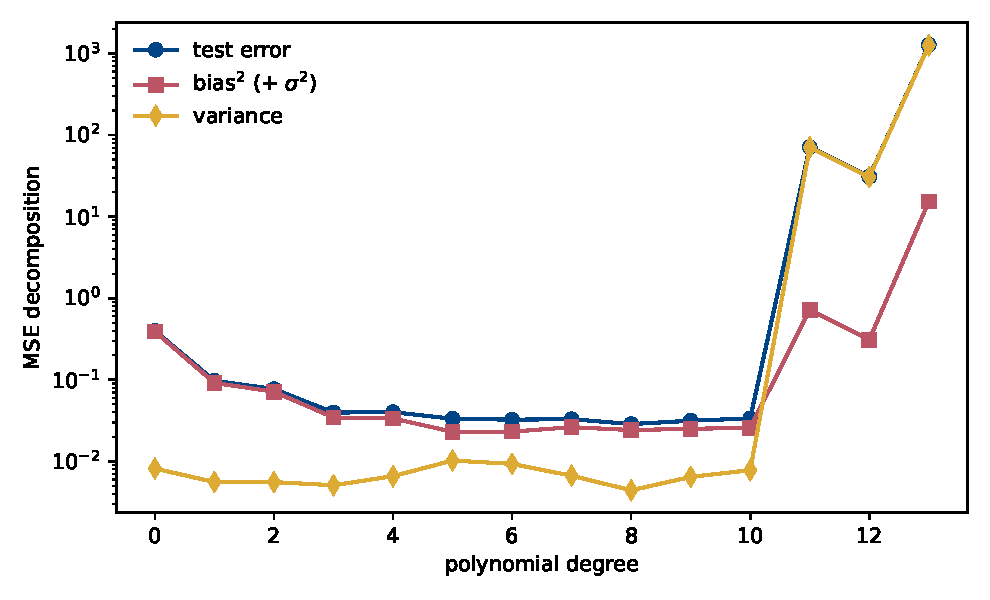
\includegraphics[width=\textwidth]{week36_bias_variance}
\end{column}
\begin{column}{0.43\textwidth}
\small
Monday's lecture closed the loop on last week's U-curve: the test error is,
by Eq.~(2.52), the sum
\[
  \mathrm{Bias}^2+\mathrm{Var}+\sigma^2,
\]
and the bootstrap let us \emph{measure} each term.  Bias falls and flattens,
variance explodes, the sum has a broad minimum (degrees 5--9 here).
\vspace{4pt}
Today you reproduce this figure yourselves, stress-test it -- more data, more
noise, a Ridge penalty -- and then let cross-validation find the minimum
without ever touching the test set, following the full recipe of
Section~3.14 for Ridge and for the Lasso.
\end{column}
\end{columns}
\end{frame}

\begin{case}[the bias-variance decomposition]
\textbf{Goal:} reproduce Monday's figure, then break it and understand the
pieces (notebook, Case 1; seed 2026 gives exactly the lecture numbers).
\begin{enumerate}
  \item Run the sweep ($n=40$, 100 bootstraps, degrees $0$--$13$) and
        reproduce \texttt{week36\_bias\_variance.pdf}.
  \item \textbf{Vary the data size:} $n=100$ and $n=400$.  Where does the
        variance explosion move?  Does the bias curve care?
  \item \textbf{Vary the noise:} $\sigma=0.3$.  Predict first, then check:
        what happens to the floor and to the minimum?
  \item \textbf{Swap the model:} replace OLS by Ridge with
        $\lambda\in\{10^{-4},10^{-1},10\}$ at fixed high degree 12.  Watch
        the variance fall and the bias rise as $\lambda$ grows -- the
        tradeoff turned into a dial.
\end{enumerate}
\vspace{2pt}
\begin{block}{Checkpoints (plenary after $\sim$25 min)}
Degree 0 has bias$^2\approx0.39$ ($\approx$ the variance of $f$ itself --
why?); the minimum is broad, degrees 5--9; at degree 13 the variance is
$\sim10^3$.  For step 4: which $\lambda$ gives the smallest \emph{total}
error at degree 12, and is it better than plain OLS at degree 6?
\end{block}
\end{case}

\begin{case}[cross-validation: choosing $\lambda$ without touching the test set]
\textbf{Goal:} a $k$-fold loop using \texttt{scikit-learn} or your own code, then used for real model selection (notebook, Case 2, steps 1--4).
\begin{enumerate}
  \item Implement 5-fold CV for Ridge on $y=3x^2+\varepsilon$ (degree-6
        polynomial, $\lambda$ on \texttt{np.logspace(-3, 5, 100)}), scaler
        fitted \emph{inside} each fold.  Reproduce
        \texttt{week36\_cv\_ridge.pdf}.
  \item Read off $\lambda^*$ and compare the minimal CV-MSE with the known
        $\sigma^2=1$.  Vary $k\in\{5,10,20\}$: how stable are $\lambda^*$ and
        the error bar (the spread over folds)?
  \item \textbf{Close the week's loop:} run CV over the polynomial
        \emph{degree} for the week-35 data set (OLS, degrees $0$--$13$) and
        compare the CV curve with Case 1's test-error curve -- same minimum,
        no test set consumed.
\end{enumerate}
\vspace{2pt}
\begin{block}{Checkpoints}
With seed 2026: $\lambda^*\approx1.2$, CV-MSE $\approx1.5$ (just above the
noise floor).  For step 3: CV picks a degree in the same broad 5--9 window as
the bootstrap decomposition, that is two independent methods, one answer.
\end{block}
\end{case}

\begin{frame}[fragile]{Case 2, continued: the full recipe of Section 3.14 -- Ridge \emph{and} Lasso}
\textbf{Goal:} turn the loop into the complete, honest procedure (notebook, steps 5--8).
\begin{enumerate}
  \setcounter{enumi}{3}
  \item \textbf{Standard error and the one-SE rule.}  Keep the spread over
        the folds, Eq.~(3.93).  Find $\lambda_{\min}$ and the largest
        $\lambda$ within one standard error of it, Eq.~(3.96).  \textbf{Refit}
        the pipeline at each on \emph{all} 100 training points and evaluate
        \textbf{once} on a fresh test set of 1000 points.
  \item \textbf{The Lasso, same data, same folds.}  Where are
        $\lambda_{\min}$ and $\lambda_{1\mathrm{SE}}$, how many of the six
        powers survive, and which?  (Mind the conventions: \texttt{Ridge}'s
        \texttt{alpha} is the book's $n\lambda$, \texttt{Lasso}'s is
        $\lambda/2$ -- Sections 3.10 and 3.14.)
  \item \textbf{Bootstrap versus cross-validation.}  Compute the training
        error, the leave-one-out bootstrap, Eq.~(3.98), and the .632
        estimator, Eq.~(3.99), for Ridge at $\lambda\in\{10^{-3},
        \lambda_{\min},\lambda_{1\mathrm{SE}},10^{3}\}$ and set them beside
        CV and the test error.  Which are optimistic, which pessimistic, and
        where does each put its minimum?
  \item \textbf{Which coefficients do you trust?}  Refit the Lasso at
        $\lambda_{\min}$ and $\lambda_{1\mathrm{SE}}$ to 200 bootstrap
        replicas and count how often each power is selected.
\end{enumerate}
\end{frame}

\begin{frame}{Case 2, continued: what you should find}
\begin{columns}
\begin{column}{0.56\textwidth}
\includegraphics[width=\textwidth]{week36_cv_ridge_lasso}
\end{column}
\begin{column}{0.42\textwidth}
\footnotesize
\begin{block}{Checkpoints (seed 2026)}
\begin{itemize}
  \item Ridge: $\lambda_{\min}\approx1.2$ (CV $1.46\pm0.21$),
        $\lambda_{1\mathrm{SE}}\approx2.1$; both refits test at $1.19$ --
        the folds cannot tell them apart, and neither can the test set.
  \item Lasso: $\lambda_{\min}\approx0.14$ keeps $x^2$ and a small $x^4$
        (test $1.03$, on the floor); $\lambda_{1\mathrm{SE}}\approx0.39$
        keeps $x^2$ \emph{alone} -- the data were $3x^2+\varepsilon$.
  \item Bootstrap: LOO-bootstrap $2.7$ and .632 $2.2$ against a test error
        of $1.19$ at $\lambda_{\min}$ -- bootstrap models see only $63\%$
        of the points; CV ($1.46$) is closer.  All put the minimum in the
        same flat valley.
  \item Stability: $x^2$ selected in $100\%$ of replicas, $x^4$ in $58\%$
        ($34\%$ at one SE) -- CV chose $\lambda$, the bootstrap says which
        coefficient to believe.
\end{itemize}
\end{block}
\end{column}
\end{columns}
\vspace{2pt}
\footnotesize
\textbf{Plenary question:} why is the CV estimate ($1.46$) \emph{above} the
test error ($1.19$) here, and why is that the safe direction to be wrong in?
\end{frame}

\begin{frame}{Wrap-up, deadlines, and Monday}
\begin{itemize}
  \item \textbf{What you should own now:} Eq.~(2.52) and what each term means
        operationally; a bootstrap loop; the selection recipe of
        Section~3.14 (leak-free folds, standard error, one-SE rule, refit,
        test set once) for Ridge and Lasso; and one sentence on why
        cross-validation, not the bootstrap, chooses $\lambda$.
  \item \textbf{Weekly exercises} (\texttt{exercisesweek36.ipynb}): the
        analytical steps of the bias-variance derivation, plus bootstrap and
        cross-validation on your own code.  Deadline \textbf{Friday
        September 4 at midnight}.
  \item \textbf{Project 1} asks for exactly today's machinery -- the code you
        wrote today is directly reusable.
  \item \textbf{Next Monday and week 38:} the main focus shifts to
<<<<<<< HEAD
                        \emph{optimization}: gradient descent methods, from plain and
                        steepest descent via momentum to stochastic gradient descent. The latter is the
=======
        \emph{optimization}: gradient descent methods, from plain and
        steepest descent via momentum to stochastic gradient descent, the
>>>>>>> main
        workhorse behind everything from Lasso to deep networks.  We will
        also briefly mention the Bayesian reading of OLS, Ridge and Lasso
        (a Gaussian prior gives Ridge, a Laplace prior the Lasso).
\end{itemize}
\begin{block}{Before you leave}
<<<<<<< HEAD
One line in an email to us: the muddiest point of
the week, what should Monday's first ten minutes next week revisit?
=======
One line in an email to us: the muddiest point of the week -- what should
Monday's first ten minutes revisit?
>>>>>>> main
\end{block}
\end{frame}

\end{document}
